\documentclass[11pt,a4paper]{article}

% ============================================================
% PACKAGES
% ============================================================
\usepackage[left=2.5cm, right=2.5cm, top=2.5cm, bottom=2.5cm]{geometry}
\usepackage[T1]{fontenc}
\usepackage{graphicx}
\usepackage{xcolor}
\usepackage{hyperref}
\usepackage{parskip}
\usepackage{enumitem}
\usepackage{booktabs}
\usepackage{fancyhdr}
\usepackage{titlesec}
\usepackage{tabularx}
\usepackage{colortbl}
\usepackage{array}
\usepackage{multirow}
\usepackage{tcolorbox}
\usepackage{tikz}
\usepackage{calc}
\usepackage{etoolbox}
\usepackage{float}

\tcbuselibrary{skins, breakable}

% ============================================================
% MRU BRAND COLOURS
% ============================================================
\definecolor{mrunavy}{RGB}{10,31,68}
\definecolor{mrublue}{RGB}{0,61,122}
\definecolor{mrumid}{RGB}{26,92,158}
\definecolor{mrusky}{RGB}{58,143,207}
\definecolor{mrugold}{RGB}{200,150,22}
\definecolor{mrupale}{RGB}{232,200,90}
\definecolor{darktext}{RGB}{45,45,45}
\definecolor{graytext}{RGB}{100,100,100}
\definecolor{lightbg}{RGB}{245,247,250}
\definecolor{alertred}{RGB}{192,57,43}
\definecolor{okgreen}{RGB}{30,140,82}
\definecolor{warnorg}{RGB}{212,123,30}
\definecolor{tabhead}{RGB}{10,31,68}
\definecolor{tabalt}{RGB}{240,244,248}

% ============================================================
% HYPERLINK SETUP
% ============================================================
\hypersetup{
    colorlinks=true,
    linkcolor=mrublue,
    urlcolor=mrublue,
    citecolor=mrublue,
    pdftitle={ODeL Strategic Proposal -- Muteesa I Royal University},
    pdfauthor={Muhindo Mubaraka},
}

% ============================================================
% SECTION FORMATTING
% ============================================================
\titleformat{\section}
    {\Large\bfseries\color{mrunavy}}{}{0em}{}[\color{mrugold}\titlerule]
\titleformat{\subsection}
    {\large\bfseries\color{mrublue}}{}{0em}{}
\titleformat{\subsubsection}
    {\normalsize\bfseries\color{mrumid}}{}{0em}{}
\titlespacing{\section}{0pt}{20pt}{8pt}
\titlespacing{\subsection}{0pt}{14pt}{6pt}
\titlespacing{\subsubsection}{0pt}{10pt}{4pt}

% ============================================================
% HEADER / FOOTER
% ============================================================
\pagestyle{fancy}
\fancyhf{}
\renewcommand{\headrulewidth}{0pt}
\fancyhead[L]{\small\color{graytext}\textit{ODeL Strategic Proposal}}
\fancyhead[R]{\small\color{graytext}\textit{Muteesa I Royal University}}
\fancyfoot[C]{%
    {\color{mrugold}\rule{\textwidth}{0.4pt}}\\[2pt]
    {\small\color{graytext} Muteesa I Royal University \quad$\vert$\quad ODeL Restoration \& Implementation Proposal \quad$\vert$\quad Page \thepage}%
}

% ============================================================
% CUSTOM ENVIRONMENTS
% ============================================================

% Highlight box (gold-accented)
\newtcolorbox{highlightbox}[1][]{
    colback=lightbg,
    colframe=mrugold,
    boxrule=0.8pt,
    left=10pt, right=10pt, top=8pt, bottom=8pt,
    fonttitle=\bfseries\color{mrunavy},
    title={#1},
    breakable,
}

% Alert box (red-accented)
\newtcolorbox{alertbox}[1][]{
    colback=red!5!white,
    colframe=alertred,
    boxrule=0.8pt,
    left=10pt, right=10pt, top=8pt, bottom=8pt,
    fonttitle=\bfseries\color{alertred},
    title={#1},
    breakable,
}

% Success box (green-accented)
\newtcolorbox{successbox}[1][]{
    colback=green!5!white,
    colframe=okgreen,
    boxrule=0.8pt,
    left=10pt, right=10pt, top=8pt, bottom=8pt,
    fonttitle=\bfseries\color{okgreen},
    title={#1},
    breakable,
}

% Navy info box
\newtcolorbox{infobox}[1][]{
    colback=mrublue!5!white,
    colframe=mrublue,
    boxrule=0.8pt,
    left=10pt, right=10pt, top=8pt, bottom=8pt,
    fonttitle=\bfseries\color{white},
    colbacktitle=mrunavy,
    title={#1},
    breakable,
}

% ============================================================
% DOCUMENT
% ============================================================
\begin{document}

% ============================================================
% TITLE PAGE
% ============================================================
\thispagestyle{empty}

\begin{center}

\vspace*{0.5cm}

% University logo
\includegraphics[height=3cm]{mru_logo.png}

\vspace{12pt}
{\color{mrugold}\rule{\textwidth}{2pt}}
\vspace{8pt}

{\fontsize{28}{34}\selectfont\bfseries\color{mrunavy}
Restoring \& Reimagining\\[4pt]
Open, Distance and e-Learning\\[4pt]
at Muteesa I Royal University}

\vspace{8pt}
{\color{mrugold}\rule{\textwidth}{2pt}}

\vspace{20pt}

{\Large\color{mrublue}\textit{A Strategic Proposal for the Vice Chancellor's Office}}

\vspace{30pt}

\begin{tabular}{r l}
    \textbf{\color{mrunavy}Prepared by:} & Muhindo Mubaraka \\[4pt]
    \textbf{\color{mrunavy}Position:} & Manager, Information Systems \\[4pt]
    \textbf{\color{mrunavy}Institution:} & Muteesa I Royal University (MRU) \\[4pt]
    \textbf{\color{mrunavy}Date:} & 12th February 2026 \\[4pt]
    \textbf{\color{mrunavy}Classification:} & \textit{Confidential --- For Internal Use Only} \\
\end{tabular}

\vspace{30pt}

{\color{mrugold}\rule{0.5\textwidth}{0.6pt}}

\vspace{12pt}

{\small\color{graytext}
Muteesa I Royal University\\
P.O. Box 14002, Kakeeka Mengo, Kampala, Uganda\\
\href{https://mru.ac.ug}{www.mru.ac.ug}}

\end{center}

\newpage

% ============================================================
% EXECUTIVE SUMMARY
% ============================================================
\thispagestyle{empty}

\section*{Executive Summary}

\begin{highlightbox}
Muteesa I Royal University's Open, Distance and e-Learning (ODeL) server has been non-functional for over two years. This proposal presents a concrete, costed, and phased plan to restore ODeL capability using cloud-hosted Moodle infrastructure---at a total annual cost of \textbf{\$2,500}---fully covered by a modest student technology fee.
\end{highlightbox}

\vspace{6pt}

Open, Distance and e-Learning (ODeL) is no longer optional in Ugandan higher education. The National Council for Higher Education (NCHE) requires every university to maintain a functional ODeL system. Peer institutions---Makerere, Kyambogo, Gulu, and Kampala International University---have invested heavily in their platforms. Meanwhile, MRU's server has been offline for two years, placing the university at regulatory risk, causing student attrition, and damaging institutional reputation.

This proposal outlines a practical solution: deploy a professionally hosted Moodle-based Learning Management System (LMS) on a cloud Virtual Private Server (VPS), complemented by custom-built integrations tailored to MRU's specific workflows and NCHE reporting requirements.

\subsection*{Key Highlights}

\begin{itemize}[leftmargin=16pt, itemsep=4pt]
    \item \textbf{Total annual cost:} \$2,500 (VPS hosting \$1,000 + development \& support \$1,000 + training \$500)
    \item \textbf{Self-sustaining revenue:} A UGX~5,000 technology fee per student per semester generates \$2,778/year at 1,000 students---exceeding all costs by \$278
    \item \textbf{Timeline:} First courses online within 90~days; full university rollout within 12~months
    \item \textbf{Architecture:} Cloud VPS with 12~CPU cores, 24\,GB RAM, 2\,TB SSD---99.9\% uptime, automated backups, enterprise security
    \item \textbf{Adoption strategy:} Five institutional policies to ensure meaningful, university-wide usage from day one
\end{itemize}

\vspace{6pt}

\noindent\textit{This document provides the Vice Chancellor with all the information needed to approve and initiate the ODeL restoration project.}

\newpage

% ============================================================
% TABLE OF CONTENTS
% ============================================================
\thispagestyle{empty}
\tableofcontents
\newpage

% ============================================================
% 1. INTRODUCTION
% ============================================================
\section{Introduction}

\subsection{Purpose of This Document}

This proposal has been prepared at the direction of the Vice Chancellor's office to address the complete breakdown of Muteesa I Royal University's Open, Distance and e-Learning (ODeL) infrastructure. It presents:

\begin{enumerate}[leftmargin=16pt, itemsep=3pt]
    \item A clear assessment of the current crisis and its consequences
    \item A detailed technical and operational solution
    \item A realistic budget with a self-sustaining revenue model
    \item A phased implementation roadmap with concrete timelines
    \item Institutional adoption policies to ensure the system is actively used
    \item A risk analysis with mitigation strategies
\end{enumerate}

\subsection{What is ODeL?}

Open, Distance and e-Learning (ODeL) is a formally recognised mode of higher education delivery in Uganda. It enables students who cannot attend traditional face-to-face classes---due to distance, employment, family responsibilities, or other commitments---to earn accredited qualifications through digital platforms.

ODeL is not merely ``putting lectures online.'' It encompasses:

\begin{itemize}[leftmargin=16pt, itemsep=3pt]
    \item \textbf{Open learning:} Flexible entry requirements and study pathways
    \item \textbf{Distance education:} Learners study remotely, with no requirement for physical presence
    \item \textbf{e-Learning:} Technology-mediated instruction, assessment, and interaction
    \item \textbf{Blended learning:} A hybrid approach combining online and occasional face-to-face sessions
\end{itemize}

\subsection{Regulatory Context}

The National Council for Higher Education (NCHE) is the statutory body responsible for regulating higher education in Uganda. Following the COVID-19 pandemic, NCHE issued Emergency Learning Guidelines and subsequently developed a comprehensive framework requiring all universities to:

\begin{itemize}[leftmargin=16pt, itemsep=3pt]
    \item Maintain a functional ODeL system capable of delivering courses remotely
    \item Develop institutional ODeL policies aligned with NCHE standards
    \item Train faculty and students in digital pedagogy and platform usage
    \item Submit regular reports on ODeL programme delivery and outcomes
\end{itemize}

\begin{alertbox}[Critical Compliance Issue]
MRU currently has \textbf{no functional ODeL system}. Every semester that passes without addressing this increases the risk of NCHE sanctions, conditions on programme accreditation, or restrictions on new programme approvals.
\end{alertbox}


% ============================================================
% 2. THE ODeL LANDSCAPE IN UGANDA
% ============================================================
\section{ODeL Across Ugandan Universities}

To appreciate the urgency of MRU's situation, it is important to understand where peer institutions stand. The table below summarises the ODeL maturity of key Ugandan universities.

\subsection{Peer Comparison}

\begin{table}[H]
\centering
\small
\renewcommand{\arraystretch}{1.4}
\begin{tabularx}{\textwidth}{>{\bfseries}l c X}
\toprule
\rowcolor{tabhead}
\textcolor{white}{\textbf{Institution}} & \textcolor{white}{\textbf{Status}} & \textcolor{white}{\textbf{Key Details}} \\
\midrule
Makerere University & \textcolor{okgreen}{Mature} &
    Institute of Open Distance and eLearning (IODeL). MUELE platform fully operational. University-wide ODeL policy framework. Staff trained. \\
\rowcolor{tabalt}
Kyambogo University & \textcolor{okgreen}{Established} &
    ODeL Centre established 2007. African Virtual University partnership. Blended learning for B.Ed programmes. Technology fee charged to students. \\
Gulu University & \textcolor{warnorg}{Launching} &
    Department of ODELL launched July 2025. Pilot: B.Ed (Primary) for 2025/2026. Target: increase enrolment from 6,000 to 11,000+. \\
\rowcolor{tabalt}
Kampala International University & \textcolor{okgreen}{Operational} &
    College of Education, Open and Distance e-Learning (CEODL) established 2011. Offers diplomas, bachelors, and masters via distance learning. \\
Muteesa I Royal University & \textcolor{alertred}{Offline} &
    Server down for 2+ years. No functional ODeL system. No distance learning capability. Non-compliant with NCHE requirements. \\
\bottomrule
\end{tabularx}
\caption{ODeL maturity comparison across Ugandan universities}
\label{tab:peer-comparison}
\end{table}

\subsection{Lessons from the Sector}

On 10th February 2026, over 51 universities convened for a national ODeL stakeholder meeting. Key themes that emerged, which directly inform this proposal, include:

\begin{enumerate}[leftmargin=16pt, itemsep=3pt]
    \item \textbf{Internet connectivity} remains the single biggest barrier. Even institutions with RENU bandwidth struggle during peak usage.
    \item \textbf{Training gaps} exist at all levels. Institutions invest in platform setup but underinvest in training lecturers and students.
    \item \textbf{Policy alignment} is needed. Existing university policies were not designed with ODeL in mind.
    \item \textbf{Cloud hosting} was recommended by multiple participants for reliability and reduced maintenance burden.
    \item \textbf{System reliability} is critical. LMS platforms that freeze during assessments cause serious academic disruption.
\end{enumerate}

\begin{highlightbox}[Insight]
MRU's proposed cloud-based approach directly addresses the infrastructure reliability and maintenance concerns raised by universities that rely on local servers. By hosting on a professional VPS, we avoid the power cuts, hardware failures, and on-site maintenance burdens that have plagued peer institutions.
\end{highlightbox}


% ============================================================
% 3. THE CURRENT CRISIS AT MRU
% ============================================================
\section{The Current Crisis at MRU}

\subsection{Situation Assessment}

MRU's ODeL server has been completely non-functional for over two years. During this period, the university has had:

\begin{itemize}[leftmargin=16pt, itemsep=3pt]
    \item \textbf{Zero online course delivery} --- no courses have been available for distance or blended learning
    \item \textbf{No digital assessment capability} --- all examinations and assignments are paper-based only
    \item \textbf{No learning management system} --- no centralised platform for course content, communication, or student tracking
    \item \textbf{No NCHE-compliant ODeL reporting} --- the university cannot demonstrate ODeL capacity to regulators
\end{itemize}

\subsection{Impact Analysis}

The consequences of this prolonged outage extend far beyond a technical inconvenience:

\begin{alertbox}[Consequences of Two Years Without ODeL]
\begin{enumerate}[leftmargin=16pt, itemsep=4pt]
    \item \textbf{Regulatory non-compliance:} NCHE requires every university to maintain a functional ODeL system. MRU's current state puts programme accreditation and new programme approvals at direct risk.

    \item \textbf{Student attrition:} Learners who need flexible, distance-based study---working professionals, students in remote areas, those with family obligations---are enrolling at competing institutions that offer online programmes.

    \item \textbf{Revenue loss:} Every student who chooses a competitor due to lack of ODeL is lost tuition revenue. Distance learning programmes also generate additional revenue with lower marginal delivery costs.

    \item \textbf{Reputational damage:} While Makerere, Kyambogo, and even newer entrants like Gulu are digitising rapidly, MRU's inability to offer any form of online learning undermines our standing among prospective students, parents, and institutional partners.

    \item \textbf{Staff frustration:} Faculty have no digital platform for course delivery. Administrative staff lack tools for student management and reporting. This contributes to low morale and limits the university's ability to attract and retain talent.

    \item \textbf{Missed partnerships and funding:} Donors, international academic partners, and research collaborators increasingly require institutions to demonstrate digital capability as a prerequisite for engagement.
\end{enumerate}
\end{alertbox}

\subsection{The Cost of Inaction}

\begin{highlightbox}[A Semester-by-Semester Loss]
Every semester that MRU operates without ODeL is not merely a missed opportunity---it is an active loss. Students enrol elsewhere. NCHE scrutiny intensifies. Competitors strengthen. The gap between MRU and its peers widens. The longer we wait, the more expensive and difficult the recovery becomes.
\end{highlightbox}


% ============================================================
% 4. THE PROPOSED SOLUTION
% ============================================================
\section{The Proposed Solution}

\subsection{Overview}

This proposal recommends deploying a \textbf{cloud-hosted Moodle-based Learning Management System (LMS)}, complemented by custom-built integrations developed specifically for MRU's workflows, administrative processes, and NCHE reporting requirements.

The solution has three layers:

\begin{table}[H]
\centering
\renewcommand{\arraystretch}{1.5}
\begin{tabularx}{\textwidth}{>{\bfseries\raggedright\arraybackslash}p{3cm} X X}
\toprule
\rowcolor{tabhead}
\textcolor{white}{\textbf{Layer}} & \textcolor{white}{\textbf{Components}} & \textcolor{white}{\textbf{Description}} \\
\midrule
\cellcolor{mrusky!12}\textcolor{mrunavy}{Users} & Students, Lecturers, Administrators & Access via browser or mobile device, from anywhere with internet connection. \\
\rowcolor{tabalt}
\cellcolor{mrublue!12}\textcolor{mrunavy}{Application} & Moodle LMS + Custom MRU Modules & Courses, assessments, grading, analytics, notifications, NCHE reporting. \\
\cellcolor{mrunavy!12}\textcolor{mrunavy}{Infrastructure} & Cloud VPS (12~CPU cores, 24\,GB RAM, 2\,TB SSD) & Automated backups, SSL encryption, 99.9\% uptime guarantee, scalable on demand. \\
\bottomrule
\end{tabularx}
\caption{Three-layer system architecture}
\label{tab:architecture}
\end{table}

\subsection{Platform Branding}

The ODeL platform requires a name that is institutional, professional, and immediately recognisable. Three options are proposed for the Vice Chancellor's consideration:

\begin{table}[H]
\centering
\renewcommand{\arraystretch}{1.5}
\begin{tabularx}{\textwidth}{>{\bfseries}l l X}
\toprule
\rowcolor{tabhead}
\textcolor{white}{\textbf{Option}} & \textcolor{white}{\textbf{Proposed Name}} & \textcolor{white}{\textbf{Rationale}} \\
\midrule
Option A & \textbf{MRU Learn} &
    Simple, clean, and institutional. Follows the naming convention used by global universities (e.g., Harvard's ``Canvas,'' Makerere's ``MUELE''). Instantly recognisable as MRU's official learning platform. \\
\rowcolor{tabalt}
Option B & \textbf{RoyalEdge} &
    Plays on ``Royal'' from Muteesa I Royal University. Conveys a modern, competitive advantage. Memorable and distinctive in Uganda's higher education space. \\
Option C & \textbf{MuteesaLMS} &
    Ties directly to the university's identity and heritage. Clear functional purpose: Muteesa's Learning Management System. Straightforward and unambiguous. \\
\bottomrule
\end{tabularx}
\caption{Proposed platform branding options}
\label{tab:branding}
\end{table}

\subsection{Why Moodle?}

Moodle is the world's most widely used open-source Learning Management System, deployed by over 300 million users across 240 countries. It is the platform of choice for most Ugandan universities, including Makerere, Kyambogo, and Mountains of the Moon University. Key advantages:

\begin{itemize}[leftmargin=16pt, itemsep=3pt]
    \item \textbf{Free and open-source:} No licensing fees, ever. The software itself costs nothing.
    \item \textbf{Proven in Uganda:} Already deployed and tested by peer institutions under similar conditions.
    \item \textbf{Highly customisable:} Can be tailored to MRU's specific academic structure, policies, and branding.
    \item \textbf{Extensive plugin ecosystem:} Thousands of plugins for plagiarism detection, video conferencing, analytics, and more.
    \item \textbf{Mobile-friendly:} Built-in responsive design and a dedicated mobile app for students on smartphones.
    \item \textbf{Active community:} Regular security updates, feature releases, and a global support community.
\end{itemize}

\subsection{Why Cloud VPS --- Not a Local Server}

MRU's previous ODeL system ran on a local, on-premise server. That server has been down for two years. This proposal specifically recommends \textbf{not} repeating that approach. The table below explains why.

\begin{table}[H]
\centering
\small
\renewcommand{\arraystretch}{1.4}
\begin{tabularx}{\textwidth}{>{\bfseries}l X X}
\toprule
\rowcolor{tabhead}
\textcolor{white}{\textbf{Factor}} & \textcolor{white}{\textbf{Local Server (Previous)}} & \textcolor{white}{\textbf{Cloud VPS (Proposed)}} \\
\midrule
Uptime &
    Subject to power cuts, UPS failures, and hardware degradation. Currently at 0\% uptime. &
    99.9\% uptime guarantee. Professional data centre with redundant power and cooling. \\
\rowcolor{tabalt}
Maintenance &
    Requires on-site IT staff, spare parts inventory, cooling systems, and physical security. &
    Fully managed by the VPS provider. MRU focuses on content and teaching, not hardware. \\
Security &
    Vulnerable to physical damage, theft, fire, and network attacks. No automated patching. &
    Enterprise-grade firewalls, SSL/TLS encryption, automated security patches, DDoS protection. \\
\rowcolor{tabalt}
Scalability &
    Fixed capacity. Upgrading requires purchasing new hardware---weeks or months of lead time. &
    Scale CPU, RAM, and storage up or down instantly based on student demand. \\
Disaster Recovery &
    No automated backups. If the server fails, data may be permanently lost. &
    Daily automated backups with geographic redundancy. Restore to any point in time. \\
\rowcolor{tabalt}
3-Year Total Cost &
    High: hardware purchase + power costs + cooling + dedicated IT staff + repairs + eventual replacement. &
    Lower total cost of ownership. Predictable monthly pricing. No capital expenditure required. \\
\bottomrule
\end{tabularx}
\caption{Cloud VPS vs.\ local server comparison}
\label{tab:vps-comparison}
\end{table}

\begin{successbox}[The Bottom Line]
A cloud VPS eliminates the exact failure mode that caused MRU's current crisis. We will never again lose our ODeL system because of a hardware failure, a power cut, or a lack of spare parts.
\end{successbox}


% ============================================================
% 5. PLATFORM CAPABILITIES
% ============================================================
\section{Platform Capabilities}

The proposed system combines Moodle's proven core functionality with custom-built integrations developed specifically for MRU.

\subsection{Core Moodle Features}

\begin{itemize}[leftmargin=16pt, itemsep=3pt]
    \item \textbf{Course content management:} Upload and organise lecture notes, readings, videos, and supplementary materials by course, topic, and week.
    \item \textbf{Assignment submission \& grading:} Students submit work digitally; lecturers grade, annotate, and return feedback---all within the platform. Full audit trail.
    \item \textbf{Discussion forums \& messaging:} Asynchronous discussion boards for each course, plus direct messaging between students and lecturers.
    \item \textbf{Video lecture hosting:} Upload recorded lectures or integrate with BigBlueButton for live virtual classes.
    \item \textbf{Online quizzes \& examinations:} Timed assessments with randomised question banks, auto-grading for objective questions, and anti-cheating measures.
    \item \textbf{Attendance \& progress tracking:} Monitor student engagement, completion rates, and activity logs.
    \item \textbf{Gradebook:} Centralised grade management with weighted categories, custom scales, and export functionality.
\end{itemize}

\subsection{Custom MRU Integrations}

Beyond Moodle's standard features, the following custom modules will be developed to address MRU's specific requirements:

\begin{itemize}[leftmargin=16pt, itemsep=3pt]
    \item \textbf{Mobile-optimised access:} Ensuring full functionality on smartphones and tablets, with a low-bandwidth mode for students with limited data.
    \item \textbf{Plagiarism detection integration:} Automated similarity checking for all submitted assignments.
    \item \textbf{SMS and WhatsApp notifications:} Critical alerts (deadlines, grades, announcements) delivered via SMS and WhatsApp, not just email---reflecting how Ugandan students actually communicate.
    \item \textbf{Administrative dashboards:} Real-time enrolment analytics, course completion rates, and departmental performance summaries for university management.
    \item \textbf{NCHE-aligned reporting:} Automated generation of reports in the format required by NCHE for ODeL compliance submissions.
    \item \textbf{Student performance analytics:} Trend analysis, early warning systems for at-risk students, and comparative performance data.
\end{itemize}


% ============================================================
% 6. INSTITUTIONAL ADOPTION POLICIES
% ============================================================
\section{Ensuring Adoption --- Institutional Policies}

Technology succeeds only when people use it. The most common failure mode for ODeL systems in Ugandan universities is not technical---it is \textit{adoption}. Platforms are deployed, but lecturers continue using paper, students never log in, and the system sits idle.

This was explicitly highlighted at the national ODeL stakeholder meeting, where Prof.\ Robert from Clarke International University noted that many institutions focus on platform setup but neglect to ensure that lecturers and students actually use the tools.

To prevent this at MRU, we propose the following five institutional policies, to be implemented in phases alongside the technical rollout:

\begin{infobox}[Policy 1: Compulsory Assignment Submission via the Platform]
All coursework assignments must be submitted through the ODeL platform. This ensures that every student and every lecturer interacts with the system regularly, and creates a verifiable digital record of all academic work. Paper submissions will no longer be accepted for coursework (examinations may remain paper-based initially).
\end{infobox}

\begin{infobox}[Policy 2: Mandatory Upload of Course Materials]
Lecturers must upload course outlines, reading lists, lecture notes, and supplementary materials to the platform at the start of each semester. This makes the ODeL system the single source of truth for all course content and ensures students always have access to up-to-date materials.
\end{infobox}

\begin{infobox}[Policy 3: Online Grade Publication]
All continuous assessment marks and final examination grades must be published through the platform. Students will check their results online, reducing administrative bottlenecks, eliminating lost result slips, and providing a permanent, auditable academic record.
\end{infobox}

\begin{infobox}[Policy 4: Course Registration via the Platform]
Course registration and semester enrolment should be processed through the ODeL system. This ensures that every student has an active account and is familiar with the platform from the very first day of each semester.
\end{infobox}

\begin{infobox}[Policy 5: Digital Attendance \& Engagement Tracking]
For programmes using blended delivery, attendance for online sessions must be tracked via the platform's built-in tools. For fully in-person programmes, the platform will track engagement through assignment submissions, forum participation, and content access---providing data-driven insights into student participation.
\end{infobox}

\begin{highlightbox}[Implementation Approach]
These policies will not be imposed overnight. They will be introduced gradually, aligned with each phase of the technical rollout: Policy~1 during the pilot phase, Policies~2--3 during the expansion phase, and Policies~4--5 during full rollout. Faculty will receive training and support before each policy takes effect.
\end{highlightbox}


% ============================================================
% 7. IMPLEMENTATION ROADMAP
% ============================================================
\section{Implementation Roadmap}

The implementation follows a three-phase approach over 12~months, designed to minimise risk and allow for iterative improvement based on real user feedback.

\subsection{Phase 1: Foundation \& Pilot (Months 1--3)}

\begin{table}[H]
\centering
\renewcommand{\arraystretch}{1.3}
\begin{tabularx}{\textwidth}{>{\bfseries}l X}
\toprule
\rowcolor{mrusky!20}
\textbf{Activity} & \textbf{Details} \\
\midrule
VPS Procurement & Procure and configure cloud VPS (12~CPU, 24\,GB RAM, 2\,TB SSD). Set up domain, SSL, and security. \\
\rowcolor{tabalt}
Moodle Installation & Install, configure, and customise Moodle with MRU branding, academic structure, and user roles. \\
Custom Development & Build priority custom modules: SMS/WhatsApp notifications, mobile optimisation, admin dashboards. \\
\rowcolor{tabalt}
Pilot Courses & Select 3--5 courses across different faculties for pilot testing with willing lecturers and their students. \\
Feedback Collection & Gather structured feedback from pilot participants. Identify issues. Iterate and improve. \\
\rowcolor{tabalt}
Policy Activation & Implement Policy~1 (compulsory assignment submission) for pilot courses only. \\
\bottomrule
\end{tabularx}
\caption{Phase 1 activities (Months 1--3)}
\end{table}

\subsection{Phase 2: Training \& Expansion (Months 4--6)}

\begin{table}[H]
\centering
\renewcommand{\arraystretch}{1.3}
\begin{tabularx}{\textwidth}{>{\bfseries}l X}
\toprule
\rowcolor{mrublue!20}
\textbf{Activity} & \textbf{Details} \\
\midrule
Faculty Training & Conduct hands-on training workshops for all lecturers: course setup, grading, content upload, forums. \\
\rowcolor{tabalt}
Student Onboarding & Orientation sessions at enrolment. Step-by-step video tutorials. SMS/WhatsApp support channel. \\
Course Expansion & Expand from pilot to 15--20 courses across all faculties. \\
\rowcolor{tabalt}
IT Helpdesk & Establish a dedicated ODeL support desk for faculty, students, and administrative staff. \\
Policy Activation & Implement Policies~2--3 (materials upload, online grades) for all expanded courses. \\
\rowcolor{tabalt}
Custom Integrations & Complete NCHE reporting module, plagiarism detection integration, and performance analytics. \\
\bottomrule
\end{tabularx}
\caption{Phase 2 activities (Months 4--6)}
\end{table}

\subsection{Phase 3: Full University Rollout (Months 7--12)}

\begin{table}[H]
\centering
\renewcommand{\arraystretch}{1.3}
\begin{tabularx}{\textwidth}{>{\bfseries}l X}
\toprule
\rowcolor{mrunavy!20}
\textbf{Activity} & \textbf{Details} \\
\midrule
Full Deployment & All programmes and courses available on the ODeL platform. Every lecturer and student has an active account. \\
\rowcolor{tabalt}
Distance Programmes & Launch first fully online distance learning programme(s), opening new student markets. \\
NCHE Reporting & Generate and submit NCHE compliance documentation demonstrating full ODeL functionality. \\
\rowcolor{tabalt}
Performance Monitoring & Continuous monitoring of system performance, student engagement metrics, and course quality. \\
Policy Activation & Implement Policies~4--5 (course registration, attendance tracking) university-wide. \\
\rowcolor{tabalt}
Knowledge Transfer & Full documentation, training of IT staff, maintenance procedures, and sustainability plan. \\
\bottomrule
\end{tabularx}
\caption{Phase 3 activities (Months 7--12)}
\end{table}


% ============================================================
% 8. TRAINING & CAPACITY BUILDING
% ============================================================
\section{Training \& Capacity Building}

The national ODeL stakeholder meeting made one thing clear: \textit{training is not optional}. Every institution that deployed an LMS without adequate training saw low adoption, frustrated users, and underutilised platforms.

MRU will invest in training for three distinct user groups:

\subsection{Faculty \& Lecturers}

\begin{itemize}[leftmargin=16pt, itemsep=3pt]
    \item Hands-on Moodle workshops (course creation, grading, forums, content upload)
    \item Online pedagogy best practices---how to teach effectively in a digital environment
    \item Ongoing helpdesk access and comprehensive written/video documentation
    \item Peer champion programme: early-adopting lecturers mentor their colleagues
\end{itemize}

\subsection{Students}

\begin{itemize}[leftmargin=16pt, itemsep=3pt]
    \item Orientation sessions integrated into the enrolment process
    \item Step-by-step video tutorials accessible on the platform and via YouTube
    \item SMS and WhatsApp support channel for quick questions and troubleshooting
    \item Printed quick-start guides for students with limited digital experience
\end{itemize}

\subsection{IT \& Administrative Staff}

\begin{itemize}[leftmargin=16pt, itemsep=3pt]
    \item System administration training: server management, updates, backups, user provisioning
    \item Monitoring and incident response procedures
    \item NCHE reporting workflows and data extraction
    \item Documentation of all custom integrations for long-term maintainability
\end{itemize}

\begin{highlightbox}[Scheduling]
Training workshops will be scheduled during existing faculty development periods and inter-semester breaks to minimise disruption to teaching. All training materials will also be available online for self-paced review and reference.
\end{highlightbox}


% ============================================================
% 9. BUDGET & REVENUE MODEL
% ============================================================
\section{Budget \& Revenue Model}

\subsection{Annual Budget Breakdown}

All costs are presented in United States Dollars (USD). The exchange rate used for UGX conversions is \textbf{1~USD = 3,600~UGX}.

\begin{table}[H]
\centering
\renewcommand{\arraystretch}{1.5}
\begin{tabularx}{\textwidth}{X r l}
\toprule
\rowcolor{tabhead}
\textcolor{white}{\textbf{Budget Item}} & \textcolor{white}{\textbf{Annual Cost (USD)}} & \textcolor{white}{\textbf{Notes}} \\
\midrule
Cloud VPS Hosting &
    \textbf{\$1,000} &
    12~CPU cores, 24\,GB RAM, 2\,TB SSD. \\
    & & Includes SSL, backups, 99.9\% uptime. \\
\rowcolor{tabalt}
System Development, Deployment \& Support &
    \textbf{\$1,000} &
    Moodle setup, custom modules, \\
    & & ongoing technical support. \\
Training \& Capacity Building &
    \textbf{\$500} &
    Faculty, student, and admin \\
    & & training workshops + materials. \\
\midrule
\rowcolor{mrunavy!10}
\textbf{Total Annual Cost} &
    \textbf{\$2,500} & \\
\bottomrule
\end{tabularx}
\caption{Annual budget breakdown}
\label{tab:budget}
\end{table}

\subsection{Revenue Model: Student Technology Fee}

To ensure the project is \textbf{self-sustaining} and does not place a recurring burden on university finances, we propose a modest student technology fee---a model already in use at Kyambogo University and other Ugandan institutions.

\begin{table}[H]
\centering
\renewcommand{\arraystretch}{1.4}
\begin{tabularx}{\textwidth}{X r}
\toprule
\rowcolor{tabhead}
\textcolor{white}{\textbf{Revenue Component}} & \textcolor{white}{\textbf{Amount}} \\
\midrule
Technology fee per student per semester & UGX 5,000 \\
\rowcolor{tabalt}
Estimated active students & 1,000 \\
Revenue per semester (1,000 $\times$ UGX 5,000) & UGX 5,000,000 \\
\rowcolor{tabalt}
Revenue per year (2 semesters) & UGX 10,000,000 \\
\midrule
\rowcolor{okgreen!10}
\textbf{Annual revenue (at 1 USD = 3,600 UGX)} & \textbf{\$2,778} \\
\bottomrule
\end{tabularx}
\caption{Revenue projection from student technology fee}
\label{tab:revenue}
\end{table}

\begin{successbox}[Self-Sustaining Model]
\textbf{Annual revenue (\$2,778) exceeds total annual cost (\$2,500) by \$278.} The project is fully self-funding from the first year. As student enrolment grows---particularly with the introduction of distance learning programmes---revenue will increase while per-student costs decrease, creating an increasingly favourable financial position.
\end{successbox}

\subsection{Financial Summary}

\begin{center}
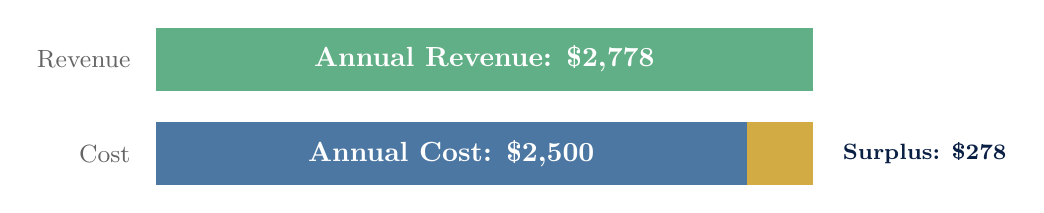
\begin{tikzpicture}
    % Revenue bar
    \fill[okgreen!70] (0,0) rectangle (8.34,0.8);
    \node[white, font=\bfseries] at (4.17,0.4) {Annual Revenue: \$2,778};
    % Cost bar
    \fill[mrublue!70] (0,-1.2) rectangle (7.5,-.4);
    \node[white, font=\bfseries] at (3.75,-0.8) {Annual Cost: \$2,500};
    % Surplus
    \fill[mrugold!80] (7.5,-1.2) rectangle (8.34,-.4);
    \node[mrunavy, font=\footnotesize\bfseries, anchor=west] at (8.6,-0.8) {Surplus: \$278};
    % Labels
    \node[graytext, font=\small, anchor=east] at (-0.2,0.4) {Revenue};
    \node[graytext, font=\small, anchor=east] at (-0.2,-0.8) {Cost};
\end{tikzpicture}
\end{center}


% ============================================================
% 10. RISK ANALYSIS & MITIGATION
% ============================================================
\section{Risk Analysis \& Mitigation}

Every project carries risk. The table below identifies the most significant risks and the specific measures we will take to address each one.

\begin{table}[H]
\centering
\small
\renewcommand{\arraystretch}{1.5}
\begin{tabularx}{\textwidth}{>{\bfseries}p{2.8cm} X X}
\toprule
\rowcolor{tabhead}
\textcolor{white}{\textbf{Risk}} & \textcolor{white}{\textbf{Description}} & \textcolor{white}{\textbf{Mitigation}} \\
\midrule
Limited Internet Access &
    Some students have poor or expensive internet connectivity, particularly in rural areas. &
    Mobile-optimised platform with low-bandwidth mode. Offline content downloads. SMS notifications for critical updates. Advocate for RENU membership. \\
\rowcolor{tabalt}
Adoption Resistance &
    Faculty or students may resist transitioning to digital tools, preferring familiar paper-based methods. &
    Hands-on training with ongoing support. Peer champions programme. Phased rollout starting with willing early adopters. Institutional policies (Section~6) that create natural usage incentives. \\
Budget Constraints &
    University may face challenges allocating resources, even at the modest levels proposed. &
    Self-funding model via technology fee eliminates recurring financial burden. Use of open-source tools avoids licensing costs. Clear ROI projections demonstrate value. \\
\rowcolor{tabalt}
Long-Term Sustainability &
    Concern that the system may deteriorate after initial setup if not properly maintained. &
    Full knowledge transfer to IT staff. Comprehensive documentation. Automated monitoring and alerting. Maintenance schedule with clear responsibilities. Cloud VPS reduces hardware maintenance to zero. \\
Staff Turnover &
    Key technical staff may leave, creating a knowledge gap. &
    All systems fully documented. Standard, widely-known technologies (Moodle, Linux). Multiple staff members trained. No proprietary or obscure tools. \\
\rowcolor{tabalt}
Data Privacy &
    Student data must be handled securely and in compliance with regulations. &
    SSL/TLS encryption for all data in transit. Encrypted backups. Role-based access controls. Data retention policies aligned with university and NCHE requirements. \\
\bottomrule
\end{tabularx}
\caption{Risk register and mitigation strategies}
\label{tab:risks}
\end{table}


% ============================================================
% 11. CONCLUSION & NEXT STEPS
% ============================================================
\section{Conclusion \& Immediate Next Steps}

\subsection{Conclusion}

MRU's ODeL system has been offline for over two years. During this time, peer universities have advanced, NCHE requirements have intensified, and MRU has lost students, revenue, and institutional standing. The situation is urgent, but it is also \textbf{entirely fixable}.

The solution proposed in this document is:

\begin{itemize}[leftmargin=16pt, itemsep=3pt]
    \item \textbf{Technically sound:} Built on Moodle, the most widely used LMS in Ugandan universities, hosted on reliable cloud infrastructure.
    \item \textbf{Financially sustainable:} A total annual cost of \$2,500, fully covered by a UGX~5,000 student technology fee with no net cost to the university.
    \item \textbf{Operationally realistic:} A phased 12-month rollout with pilot testing, structured training, and iterative improvement.
    \item \textbf{Strategically valuable:} Positions MRU alongside Makerere, Kyambogo, and Gulu as a digitally capable institution, opens new student markets, and ensures NCHE compliance.
\end{itemize}

\subsection{Immediate Next Steps}

We respectfully request the Vice Chancellor's approval to proceed with the following actions:

\begin{enumerate}[leftmargin=16pt, itemsep=6pt]
    \item \textbf{Formal approval} to proceed with the ODeL restoration project as outlined in this proposal.
    \item \textbf{Establish an ODeL Task Force} with representation from IT, faculty, and administration to oversee implementation.
    \item \textbf{Approve the UGX 5,000 technology fee} to provide a self-sustaining funding mechanism for the project.
    \item \textbf{Procure cloud VPS hosting} and a professional domain name for the platform.
    \item \textbf{Begin Phase~1 pilot implementation}---first courses online within 90~days of approval.
    \item \textbf{Schedule monthly progress reviews} with the Vice Chancellor's office to ensure accountability and transparency.
\end{enumerate}

\vspace{12pt}

\begin{highlightbox}
\centering
\textit{\large``This is not just about fixing a server.\\[4pt]
It is about positioning Muteesa I Royal University\\[4pt]
for the future of higher education in Uganda.''}
\end{highlightbox}


% ============================================================
% SIGNATURE
% ============================================================
\vspace{24pt}

\noindent{\color{mrugold}\rule{\textwidth}{0.6pt}}
\vspace{8pt}

\noindent\textbf{Prepared and submitted by:}

\vspace{6pt}

\noindent\includegraphics[height=1.2cm]{muhindo_signature.png}

\vspace{4pt}

\noindent\textbf{Muhindo Mubaraka}\\
Manager, Information Systems\\
Muteesa I Royal University

\vspace{4pt}

\noindent\textbf{Date:} 12th February 2026

\vspace{4pt}

\noindent\textbf{Contact:}\\
Email: mubahood360@gmail.com\\
Phone: +256 783 204 665 / +256 706 638 484

\end{document}
